\documentclass[11pt,a4paper]{article}

\usepackage[english]{babel}
\usepackage[T1]{fontenc}
\usepackage[utf8]{inputenc}
\usepackage{graphicx}
\graphicspath{{../Figs/}}
\usepackage{float}
\usepackage{subcaption}
\usepackage[font=footnotesize,labelfont={sf,bf},textfont=sf,width=\textwidth]{caption}
\usepackage[margin=2cm]{geometry}
\usepackage[plainpages=false,pdfpagelabels,hypertexnames=false]{hyperref}
\usepackage[usenames,dvipsnames]{xcolor}
\usepackage{mathtools}
\usepackage[separate-uncertainty=true, multi-part-units=single]{siunitx}
\usepackage{booktabs}
\usepackage{physics}
\usepackage[bottom]{footmisc}

\title{\bfseries\textsc{Holography}}
\author{
Michele Masini\\ \small\texttt{\href{mailto:michele.masini@uni-ulm.de}{michele.masini@uni-ulm.de}}\and
Iyán Méndez Veiga\\ \small\texttt{\href{mailto:iyan.mendez-veiga@uni-ulm.de}{iyan.mendez-veiga@uni-ulm.de}}
}
\date{\today}


\begin{document}
\maketitle

\begin{abstract}
Holography experiments are not common in bachelor laboratories. Our motivation for doing this experiment was to understand the theory of holography, and to create and observe some holograms for the first time.

In the experiment we created four holograms. In the following report, holography is briefly explained theoretically and the experimental setup and procedures are described in detail. Pictures of the obtained holograms are shown, as well as results from two holographic interferometry measurements.
\end{abstract}


\section{Introduction}

In conventional imaging techniques, such as photography, what is recorded is merely the intensity distribution in the original scene. As a result, all information about the optical paths to different parts of the scene is lost.

The unique characteristic of holography is the idea of recording both the phase and the amplitude of the light waves from an object. But since all recording materials respond only to the intensity in the image, it is necessary to convert the phase information into variations of intensity.

The purpose of this report is to show, both theoretical and experimentally, how this can be achieved using coherent light.

We will start from the very beginning and the foundation of classical electromagnetism: the Maxwell equations. Then, we will describe how EM fields propagate by derivating the wave equation from the Maxwell equations and write some of its solutions. We will also see the implications of the superposition principle and what we mean by coherent light. A brief summary of the physics of lasers will be presented and, finally, holography will be explained. Additionally, we will describe the experimental procedure to create the holograms, and at the end we will show the obtained holograms.


\section{Theory}

\subsection{Maxwell equations}

Maxwell equations \cite{feynman} are a set of linear differential equations that describe how electric and magnetic fields are generated by charges, currents, and changes of the fields. Together with the Lorentz force, $\vb{F}=q(\vb{E}+\vb{v}\times\vb{B})$, form the foundation of classical electromagnetism.

The complete Maxwell equations are the following:

\begin{subequations}\label{eq:maxwell_equations}
\begin{align}
&\div\vb{E}=\frac{\rho}{\epsilon_0}\label{eq:maxwell_1}\\
&\curl\vb{E}=-\pdv{\vb{B}}{t}\label{eq:maxwell_2}\\
&\div\vb{B}=0\label{eq:maxwell_3}\\
&\curl\vb{B}=\frac{1}{c^2}\qty(\frac{\vb{j}}{\epsilon_0}+\pdv{\vb{E}}{t})\label{eq:maxwell_4}
\end{align}
\end{subequations}

The first equation \eqref{eq:maxwell_1}, read as \emph{the divergence of $\vb*{E}$ is the charge density over $\epsilon_0$}, is the differential form of the Gauss' law, which is always valid both in dynamic and static fields. Equivalently, in the integral form it means that the flux of the electric field through a closed surface is equal to the charge inside that surface over the vacuum permittivity, i.e. the capability of the vacuum to permit electric field lines.

The third equation \eqref{eq:maxwell_3} is the corresponding general law for magnetic fields. That the divergence of the magnetic field is zero is the mathematical way of expressing that magnetic monopoles cannot be found in nature.

The second equation \eqref{eq:maxwell_2}, that \emph{the curl of $\vb*{E}$ is -$\pdv*{\vb*{B}}{t}$}, is the differential form of the Faraday's law. The line integral of the electric field around a loop is equal to minus the derivative with respect to time of the flux of the magnetic field through that loop.

Last equation \eqref{eq:maxwell_4}, when Maxwell wrote it down, included new physics. He added a new term when he noticed something strange in the expression that was used before to explain magnetic fields produced by steady currents $\curl\vb{B}=\vb{j}/(c^2\epsilon_0$). Taking the divergence on both sides, the left-hand side is zero\footnote{The divergence of a curl is always zero.}, and if we want the equation to be true then we require that the divergence of $\vb{j}$ is also zero. This means that the total flux of current out of any closed surface has to be zero, and this makes no sense since we know that charges can move from one place to another. Maxwell's solution was to add the extra term $\pdv*{\vb{E}}{t}$ to the right-hand side, which became his fourth and last equation.

In the integral form, we can read the fourth equation as: the integral of the magnetic field around a loop is proportional, being the proportionality constant one over the speed of light squared, to the current through the loop over the vacuum permittivity plus the derivative with respect to time of the flux of the electric field that goes through the same loop.

If we accept Maxwell's equations, and we should since no one has ever found an experiment that disagrees with them, we must conclude that charge is always conserved. Conversely, if we assume that the electric charge is conserved, and we write this fundamental law as $\div\vb{j}=-\pdv*{\rho}{t}$, meaning that any flow of charge must come from some supply, then this is exactly the term that Maxwell had to add to straighten out the difficulty we found.

\subsection{Wave equation}

By means of the Maxwell equations, it is possible to describe the propagation of light as the propagation of a wave called electromagnetic wave. It is not hard to imagine that light does not carry charge, hence we will suppose $\rho=0$ and $\textbf{j}=0$.

In this conditions, Maxwell's equations read:
\begin{subequations}\label{eq:maxwell_equations_wo_charge}
\begin{align}
&\div\vb{E}=0\label{eq:maxwell__wo_1}\\
&\curl\vb{E}=-\pdv{\vb{B}}{t}\label{eq:maxwell_wo_2}\\
&\div\vb{B}=0\label{eq:maxwell_wo_3}\\
&\curl\vb{B}=\frac{1}{c^2}\qty(\pdv{\vb{E}}{t})\label{eq:maxwell_wo_4}
\end{align}
\end{subequations}

We can decouple the previous equations using the following rule:
\begin{equation}
\curl \curl \vb{F}=\nabla (\div \vb{F})- \nabla^2\vb{F}\label{rule}
\end{equation}
where $\vb{F}$ is a generic field. Let us apply for instance equation (\ref{eq:maxwell_wo_3}) and (\ref{eq:maxwell_wo_4}) to (\ref{rule}) to get:
\begin{align*}
\curl \curl \vb{B} &=\nabla (\div \vb{B})- \nabla^2\vb{B} \\
\curl \frac{1}{c^2}\qty(\pdv{\vb{E}}{t}) &=0-\nabla^2\vb{B} \\
\frac{1}{c^2}\qty(\pdv{\curl \vb{E}}{t}) &=-\nabla^2\vb{B}
\end{align*}
Finally, using (\ref{eq:maxwell_wo_2}):
\begin{equation}
\nabla^2\vb{B}=\frac{1}{c^2}\pdv{^2 \vb{B}}{t^2}
\end{equation}
Analogously for the electric field, we obtain:
\begin{equation}
\nabla^2\vb{E}=\frac{1}{c^2}\pdv{^2 \vb{E}}{t^2}
\end{equation}
We have obtained two three-dimensional wave equations. The general solution is of the form:
\begin{align}
\vb{B}(\vb{r},t) &=\vb{B_0}e^{i(\vb{k} \cdot \vb{r}-\omega t+\phi_0)}\\
\vb{E}(\vb{r},t) &=\vb{E_0}e^{i(\vb{k} \cdot \vb{r}-\omega t+\phi_0)}\label{elec}
\end{align}
If we suppose that the wave is propagating only along z, we have:
\begin{align}
\vb{B}(z,t) &=\vb{B_0}e^{i(kz-\omega t+\phi_0)}\\
\vb{E}(z,t) &=\vb{E_0}e^{i(kz-\omega t+\phi_0)}
\end{align}
Using equation (\ref{eq:maxwell__wo_1}) and (\ref{eq:maxwell_wo_3}), we can see that the z-component of the fields is zero. Moreover, using equation (\ref{eq:maxwell_wo_2}), we easily notice that magnetic and electric field have to be orthogonal.

\subsection{Superposition principle}

Let us suppose that we have 2 waves of the form (\ref{elec})\footnote{We call $\phi_{1,2}(t)\equiv\vb{k_{1,2}} \cdot \vb{r}-\omega_{1,2} t+\phi_0$}. We will see what an observer would measure looking at the superposition between the two waves. What we are going to measure in a laboratory is the intensity of light, where $I\propto \abs{\vb{E}}^2$.

In our case:
\begin{align*}
I_{TOT}\propto \abs{\vb{E_1}+\vb{E_2}}^2 &=\abs{\vb{E_{0,1}}e^{i\phi_1}+\vb{E_{0,2}}e^{i\phi_2(t)}}^2\\
&=\abs{\vb{E_{0,1}}}^2+\abs{\vb{E_{0,2}}}^2+\vb{E_{0,1}}\cdot \vb{E_{0,2}}e^{i\phi_1}e^{-i\phi_2(t)}+\vb{E_{0,2}}\cdot \vb{E_{0,1}}e^{i\phi_2(t)}e^{-i\phi_1(t)}
\end{align*}
Finally, using Euler's formula we get:
\begin{equation}
I_{TOT}(t)\propto I_1+I_2+2\vb{E_{0,1}}\cdot \vb{E_{0,2}}cos(\phi_1(t)-\phi_2(t))
\end{equation}
We can notice that there is a superposition term in the result. This term is responsible of the so called \emph{interference}, i.e. constructive (when $cos(\Delta\phi)>0$) or distructive (when $cos(\Delta\phi)<0$) superposition of the two waves.  Anyway, it is really hard to observe this term because, during an experiment, we measure the avarage of the intensity over a certain interval of time:
\begin{align*}
I_{AV} &= \frac{1}{t_{max}}\int_0^{t_{max}}I(t)dt\\ &\propto I_1+I_2+ 2\vb{E_{0,1}}\cdot \vb{E_{0,2}} \frac{1}{t_{max}} \int_0^{t_{max}} cos(\phi_1(\vb{r},t)-\phi_2(\vb{r},t)) dt\xrightarrow{t_{max}\rightarrow \infty} I_1+I_2
\end{align*}


\subsection{Coherence}
When we speak about \emph{coherence of light}, we are referring to two or more waves whose phase difference $\Delta\phi(\vb{r},t)\equiv \phi_1(\vb{r},t)-\phi_2(\vb{r},t)$ is constant in space and time:
\begin{equation}
\Delta\phi(\vb{r},t)=\Delta\phi_0
\end{equation}
A second reason why we do not observe interference in everyday life is the fact that the superposition term varies too fastly because of the non-coherence nature of light coming from natural sources.

We will introduce two kinds of coherence: temporal and spatial coherence. We speak about the former when we start with two equal waves, we introduce a retardation in one of them (let us say $\tau_0$) and we observe their superposition. We will have a phenomenon of interference due to their pase difference $\omega \tau_0$ and we will call \emph{coherence lenght} the difference of optical path between the two waves: $l_c\equiv c\tau_0$.

As far as spatial coherence is concerned, it arises when two fields arrive in two different points of space. This will cause a phase difference.

\subsection{Physics of lasers}

Laser (\emph{L}ight \emph{A}mplification by \emph{S}timulated \emph{E}mission of \emph{R}adiation) take advantage of the phenomenon of spontaneous emission. However, to fully understand how a laser works we need to consider other two phenomena: spontaneous emission and absorption.

\begin{figure}[ht]
\centering
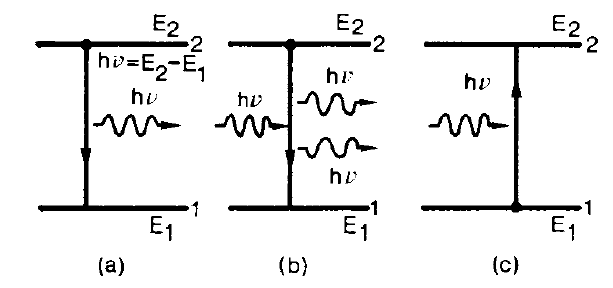
\includegraphics[width=.6\textwidth]{TLS}
\caption{Schematic illustration of the three processes that a TLS can experience that involve photons: (a) spontaneous emission, (b) stimulated emission, and (c) absorption \cite{svelto2010principles}.}
\label{fig:2LS}
\end{figure}

\paragraph{Two-level systems}
Let us consider a two-level system (TLS) with energies $E_1$ and $E_2$ ($E_1<E_2$). We will call the level with energy $E_1$ the ground state, and the level with energy $E_2$ the excited state, although these two levels could by any two out of the infinite discrete set of levels that a system may have. If at a certain time, the system is in the excited state, it will tend to decay to the ground state since $E_2>E_1$. When this happens, a photon is emitted with energy $h\nu_0=E_2-E_1$. This process is called \emph{spontaneous emission}. To emphasize that a photon is emitted it is also called \emph{radiative emission} since other decay channels exist that may not involve photons at all (e.g. phonons) but these processes are called \emph{non-radiative} decays. However, if we have an incident photon with energy $hv_0=E_2-E_1$, there is a probability that this photon will stimulate the system to decay to the ground state. This process is called \emph{stimulated emission} and it looks similar to the spontaneous emission but there is a fundamental difference: the emitted photon in the stimulated emission process has the same phase and direction of the external one while in the case of radiative emission, photons are emitted with random phase and direction. Finally, considering the same incident photon but now with the system in the ground state, there is also the probability that the system will absorb the photon which allows the transition to the excited level. This process is called \emph{absorption}. These three processes are shown in Figure \ref{fig:2LS}.

To compute the probabilities of these processes we need to know the population of each atom state. If we define this population $N_i(t)$ as the number of atoms per unit volume at a certain time $t$ that are in the energy level $i$, then we can write the following equation for the spontaneous emission process:

\begin{equation}\label{eq:spontaneous_emission}
\left(\frac{dN_2(t)}{dt}\right)_{sp}=-A_{21}N_2(t)=-\frac{N_2(t)}{\tau_{sp}}\,,
\end{equation}
where $A_{21}$ is called the Einstein $A$ coefficient\footnote{For historical reasons. Einstein obtained an expression for A from thermodynamic considerations.} and $\tau_{sp}=1/A_{21}$ is called the spontaneous emission (or radiative) lifetime. In the case of radiative emission, this coefficient only depends on the particular transition.

Similarly, for the stimulated processes we have the following expressions:

\begin{align}\label{eq:stimulated_emission}
\left(\frac{dN_2(t)}{dt}\right)_{st}&=-B_{21}N_2(t)\\ \label{eq:absorption}
\left(\frac{dN_1(t)}{dt}\right)_{st}&=-B_{12}N_1(t)\,,
\end{align}
where $B_{21}$ is called rate of stimulated emission or Einstein $B$ coefficient. In this case, this constant does not only depend on the particular transition but also on the intensity of the incident wave. To avoid this dependence, it is quite common in the literature to write the rate equation in terms of $B_{21}=\sigma_{21}F$, which is a valid expression for plane waves where $\sigma_{21}$ is the cross section of the process and $F$ the photon flux. Similarly, $B_{12}$ is called the absorption rate and it can also be written as $B_{12}=\sigma_{12}F$. The advantage in that both cross sections only depend on the particular transition like the $A$ coefficient.

Einstein showed that in the case of non-degenerate TLS, it is always true that $B_{12}=B_{21}$ or, equivalently,  $\sigma_{12}=\sigma_{21}$. He also showed that if level 1 and level 2 are $g_1$-fold $g_2$-fold degenerate respectively, then $g_1B_{12}=g_2B_{21}$ or, equivalently, $g_1\sigma_{12}=g_2\sigma_{21}$.

The reason for the key condition of population inversion that we need to have a laser can be understood with this simple TLS. Let us suppose that we have a certain material composed of many atoms or molecules that can be model with our simple TLS model and we have an incident plane wave travelling a distance $dz$ through this material. It is possible to obtain (and it is done in detail in \cite{svelto2010principles}) that the flux difference $dF$ after the distance $dz$ is given by
\begin{equation}\label{eq:dF}
dF=\sigma_{21}F\left(N_2-\frac{g_2}{g_1}N_1\right)
\end{equation}

When $dF$ is positive, the material behaves as an amplifier and it is called an active material, and when it is negative, it behaves as an absorber. The condition we found is the following
\begin{equation}
dF>0\;\Leftrightarrow\;N_2-\frac{g_2}{g_1}N_1>0\;\Leftrightarrow\;N_2>\frac{g_2}{g_1}N_1\,,
\end{equation}
which is the so-called \emph{population inversion} condition.

Note that at thermal equilibrium, $dF<0$ because populations are described by Boltzmann statistics and we have that
\begin{equation}
\frac{N_2^\text{eq}}{N_1^\text{eq}}=\frac{g_2}{g_1}\exp\left[-\frac{E_2-E_1}{k_BT}\right]<1
\end{equation}
and also that, for a TLS, the best non-equilibrium condition that we can reach is $N_2=N_1$ because at that point absorption and stimulated emission processes compensate between each other. Hence, it is not possible to achieve population inversion with a TLS, and to build lasers we need to consider three and four level systems like the ones shown in Figure \ref{fig:3LS-4LS}.

\begin{figure}[ht]
\centering
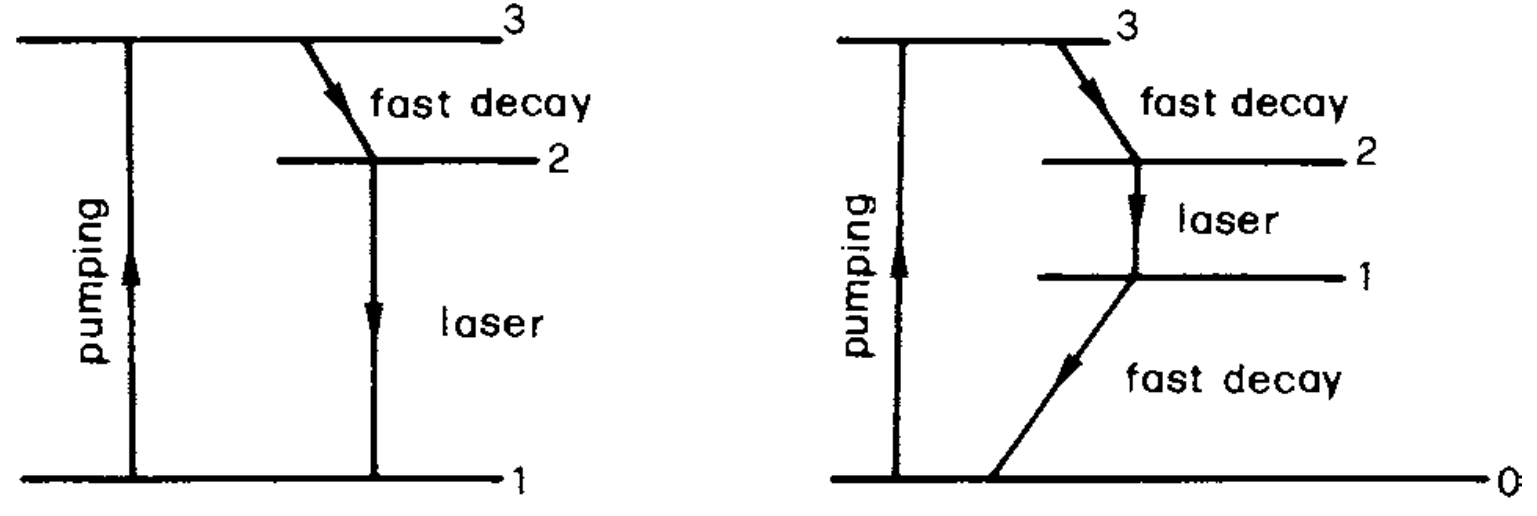
\includegraphics[width=0.7\textwidth]{3LS-4LS}
\caption{Schematic illustrations of a three-level system (left) and a four-level system (right) \cite{svelto2010principles}. Excitation of the system is always from the lowest energy level to the highest one, but there is an extra level between the laser transition and the ground state in the case of the four-level system. Population inversion is achievable in both scenarios with a proper pumping mechanism.}
\label{fig:3LS-4LS}
\end{figure}

\paragraph{Three and four-level systems}
In the case of the three-level system laser, atoms are excited somehow by a pumping mechanism from level 1 to level 3. Then, there is a fast non-radiative decay (e.g. via phonons) from level 3 to level 2, and due to this fact the population inversion is achieved between levels 1 and 2. Photons with the energy of this transition are amplified when this condition is reached.

In the case of the four-level system, atoms are excited from the level 0 to the level 3. Again, there is a fast non-radiative decay from level 3 to level 2, but the main difference with respect to the three-level system is that the laser transition is not between this level and the ground state, but there is an extra level (level 1) which also has a non-radiative decay to the ground state.

Population inversion can be achieved in both schemes, so the reason to consider four-level systems instead of just settling for the three-level system is because it is easy to produce a population inversion. Although this can be proved rigorously studying the rate equations for both cases, it is also possible to understand it in an intuitive way.

When by using the pumping mechanism we raise one atom from level 1 to level 3 in the case of a three-level system, we can assume that if the non-radiative decay is fast enough, the atom will be «immediately» in the level 2. Level 3 is, therefore, empty. Let us also suppose that $g_1=g_2$ to simplify the maths and make the point. By looking at expression \eqref{eq:dF}, we see that to compensate the absorption with the stimulated emission in the laser transition, we need to get at least to $N_2=N_1$ by pumping atoms from the ground state to the level 3. Only at that point, the following atoms that are raised contribute to get the population inversion, and we start to observe an amplification of the light.

However, in the case of a four-level systems, since there is second non-radiative fast decay channel from level 1 to level 0, level 1 can be consider to be always empty and any atom pump to level 3 will contribute to the population inversion of the laser transition. This means that less power is needed for the pumping mechanism in the case of a four-level system.

\paragraph{Oscillator}
We have seen that it is possible to reach the population inversion with three and four-level systems. Assuming that we succeed in finding both a material that can be model with these schemes and also a pumping mechanism, then we end up with a material that amplifies incoming photons in resonance with that transition. However, to build a laser we are still missing one component: a resonance cavity or oscillator.

\begin{figure}[ht]
\centering
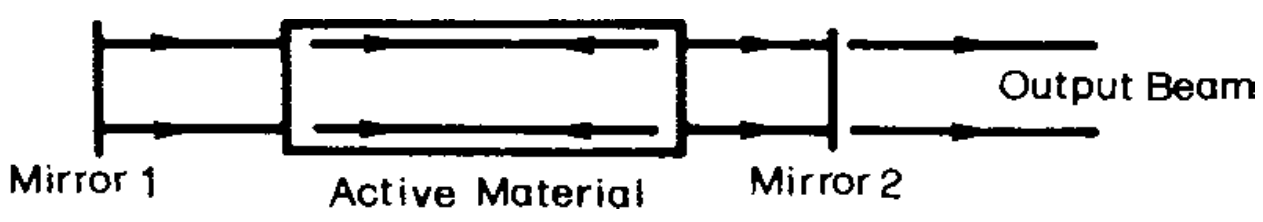
\includegraphics[width=0.5\textwidth]{laser}
\caption{Scheme of a laser. An active material excited with a pumping mechanism enclosed in a a resonance cavity. Light gets amplified by crossing the active material and escapes the oscillator through the second mirror (asumming $R_2<R_1$) \cite{hariharan_2002}}
\label{fig:laser}
\end{figure}

This is done by enclosing the active material between two highly reflective mirrors, with one of them slightly more transparent than the other. After a critical point, where the loses due to the output coupling (photons that leave the cavity or are absorbed by the mirrors) are compensated by the gain in the active medium, more and more photons are amplified every time they cross the active material, and we obtain the amplified light beam, i.e. laser, escaping from the less reflective mirror as shown in Figure \ref{fig:laser}.

To sum up, four requirements are needed to build a laser: an active material or, as it is usually called, a gain medium; a pumping mechanism to get excite this medium and fulfil the population inversion condition; a resonator or oscillator; and an outcoupling to get an output beam from the cavity (typically a partially transparent mirror).

\paragraph{Properties of lasers} All this effort is justified by the unique properties of laser radiation. Laser light is characterized by an extremely high degree of monochromaticity,  coherence, directionality, and brightness. Moreover, although perhaps a less fundamental property, it is possible to produce very short light pulses, very important for some scientific applications and out of reach for other light sources.

\subsection{Holography}\label{sec:Holo}

As it was advanced in the introduction, holography is a technique to capture in a photosensitive material, the amplitude and phase of the light, in order to produce 3D images. This gain in information when we compare to photography is not free of cost: both creating (Figure \ref{fig:hologram_recording}) and observing (Figure \ref{fig:hologram_reconstruction}) holograms involve a more complex setup than traditional cameras, and also the use of coherent light like the one produced by lasers.

\begin{figure}[ht]
\centering
\begin{subfigure}[b]{0.48\textwidth}
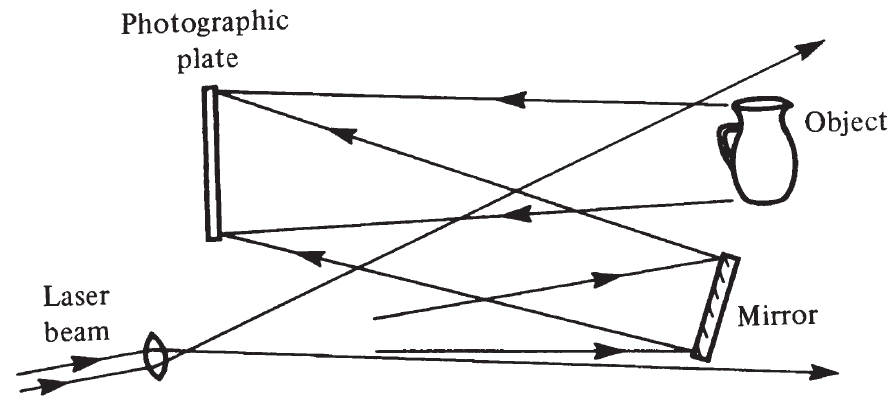
\includegraphics[width=\textwidth]{Hologram_recording}
\caption{}
\label{fig:hologram_recording}
\end{subfigure}
\begin{subfigure}[b]{0.48\textwidth}
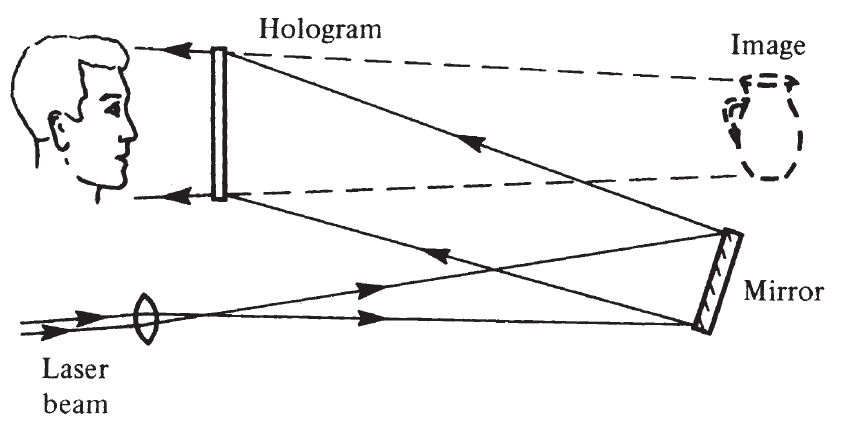
\includegraphics[width=\textwidth]{Hologram_image_reconstruction}
\caption{}
\label{fig:hologram_reconstruction}
\end{subfigure}
\caption{In \ref{fig:hologram_recording}, a diagram of the hologram recording setup. The interference pattern produced by the reference wave and the object wave is recorded. In \ref{fig:hologram_reconstruction}, Diagram of the image reconstruction. Light diffracted by the hologram reconstructs the original object wave.\cite{hariharan_2002}}
\label{fig:holograms}
\end{figure}

Holography was first demonstrated by Gabor in 1948 with a collimated beam of monochromatic light (not a laser). With the invention of lasers, which provided a new source of coherent light, holography has evolve a lot. Many variations of the original idea appeared in the following years, such as holographic interferometry, holographic microscopy, holographic tomography, etc.


\paragraph{Holographic interferometry}
Moreover, thanks to holography, it is possibole to get information about the optical path of the light. As we have said, an hologram contains also information about the phase of light. If we know the phase difference of two coherent beams, we can derive the optical path. In fact, when the wavelength is constant, we can express the phase difference as:
\begin{equation}
\Delta \phi=kD=\frac{2\pi}{\lambda}D\label{eq:Delphi}
\end{equation}
where $D$ is the difference of the optical path between the first and the second beam.

Let us suppose that in our experiment we move the reflecting object of a distance $d$. If the distance from the photosensitive plate and the object is much greater than $d$, then we can consider the angle between the incoming and outgoing beam unchanged. Let $\theta_1$ and $\theta_2$ be the angles between the incoming (1) and outgoing (2) beam and the normal to the object surface, then: 
\begin{equation}
D\simeq d(cos\theta_1+cos\theta_2)\label{eq:D}
\end{equation}

By exposing the photosensitive plate two times, before and after the movement of the object, we will observe a certain number $N$ of interference fringes on the moved object. Knowing $\Delta \phi=2\pi N$, equating it with equation (\ref{eq:Delphi}) and using equation~(\ref{eq:D}), we get:
\begin{equation}
d\simeq\frac{N\lambda}{cos\theta_1+cos\theta_2}\label{eq:d}
\end{equation}

If, instead of moving the object, we rotate it a small angle $\alpha$, we can state that
\begin{equation}
d\simeq R\alpha
\end{equation}
where $R$ is the radius of the rotation. Therefore, we can extimate the angle $\alpha$ with good precision
\begin{equation}
\alpha\simeq \frac{N\lambda}{R(cos\theta_1+cos\theta_2)}\label{eq:alp}
\end{equation}

\section{Experimental procedure}

\paragraph{Optical setup}
The first thing we had to do was adjust the optical bench. Almost everything was already set up but we did have to align the objective and the spatial filter for the reference beam. These optical elements are placed just after the beam splitter in the path of the reference beam (see Figure \ref{fig:optical_bench_1}). First we aligned the backside of the objective with the help of a small paper sheet. Then we put the spatial filter just after it and use the screws to align it at exactly where the beam was focused. Transversal alignment was done by trying to find the maximum of light through the spatial filter. Once we did that, we move the spatial filter in the longitudinal direction till the Airy pattern due to diffraction from the optical system's aperture disappeared and we had a clear Gaussian beam.

\begin{figure}[ht]
\centering
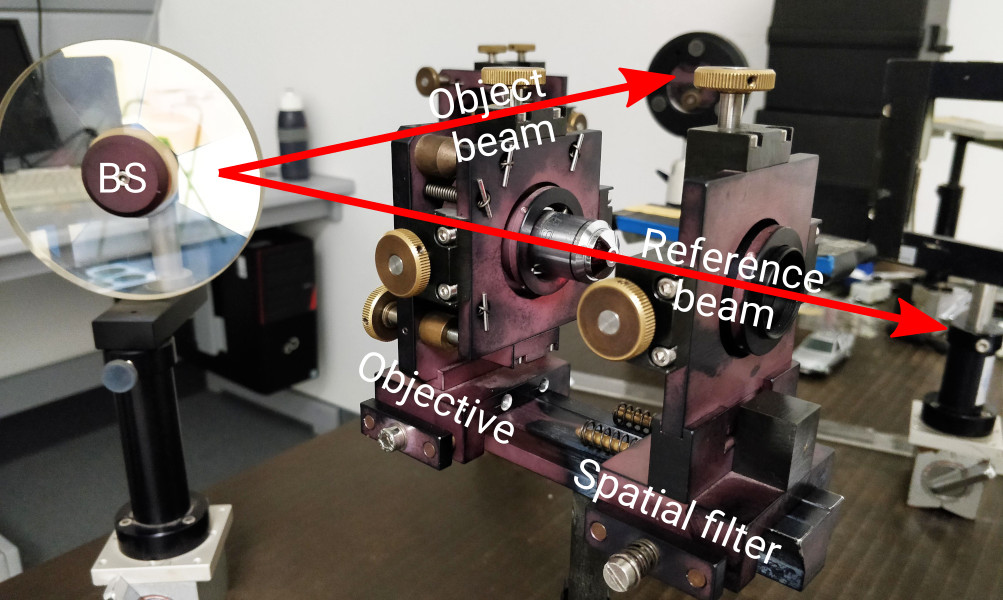
\includegraphics[width=0.75\textwidth]{Optical_bench_1}
\caption{The BS divides the laser in two beams: the reference and the object beam. Reference beam goes through an objective and a spatial filter in order to obtain a Gaussian beam, which is reflected by a mirror to the photosensitive plate.}
\label{fig:optical_bench_1}
\end{figure}

\paragraph{Mixing of chemicals}
In order to observe the hologram, we needed to protect the photosensitive material from light once we exposed it to the desired object. This was done by using a negative developer and a rapid fixer. We prepared two solutions using the the chemicals produced by \href{https://www.tetenal.com/}{Tetenal}. We prepared \SI{1}{\litre} of developer by mixing \SI{200}{\milli\litre} of the ultrafin with \SI{800}{\milli\litre} of water. We also prepared \SI{1}{\litre} of fixer with \SI{150}{\milli\litre} of the superfix plus and \SI{850}{\milli\litre} of water.

%\begin{figure}[ht]
%\centering
%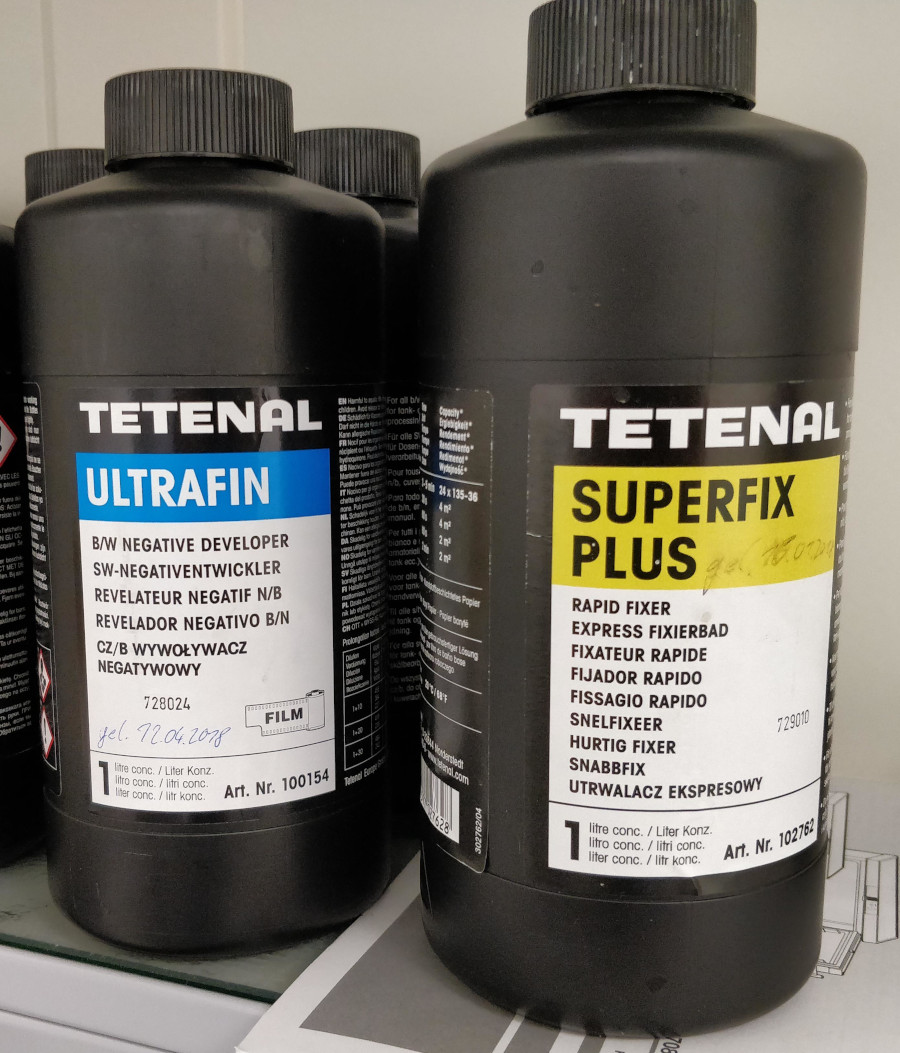
\includegraphics[width=0.3\textwidth]{Chemicals}
%\caption{The negative developer and the rapid fixer used to prepare the two dilutions.}
%\label{fig:chemicals}
%\end{figure}

The procedure to expose, develop and fix the photosensitive plate was the following: \SI{90}{\second} of exposure to the object and reference beams, \SI{2}{\min} bath in the developer dilution, \SI{10}{\second} bath in water, \SI{4}{\min} bath in the fixer dilution, and finally \SI{2}{\min} bath in water. After this, the plates were put to dry next to a fan.

\paragraph{Hologram creation}
An object is illuminated by the object beam and the reflected light reaches the photosensitive plate. Simultaneously, the reference beam illuminates directly the photosensitive plate in order to obtain an interference pattern. For creating the hologram, the beam splitter is put in the 95-5 position, so 5\% of the intensity of the light goes to the reference path and 95\% illuminates the object.

\paragraph{Holography interferometry}
In order to see interference fringes in the hologram, instead of the long single \SI{90}{\second} exposure mentioned before, we used two \SI{45}{\second} exposures, and we moved the object, by either a very small distance or an angle, after the first exposure.

Number of fringes were obtained using \href{https://imagej.net/}{ImageJ}. Images were first desaturated and then the profile of a line crossing all the fringes was plotted. By counting the peaks we determined the number of fringes.

\section{Results and conclusions}

We created three holograms. In the first one, we reproduced the figure of a car with a chess piece on the bonnet. Following the procedure explained in the previous section, we got the image shown in Figure~\ref{fig:off_axis_hologram1}.
\begin{figure}[ht]
\centering
\begin{subfigure}[b]{0.45\textwidth}
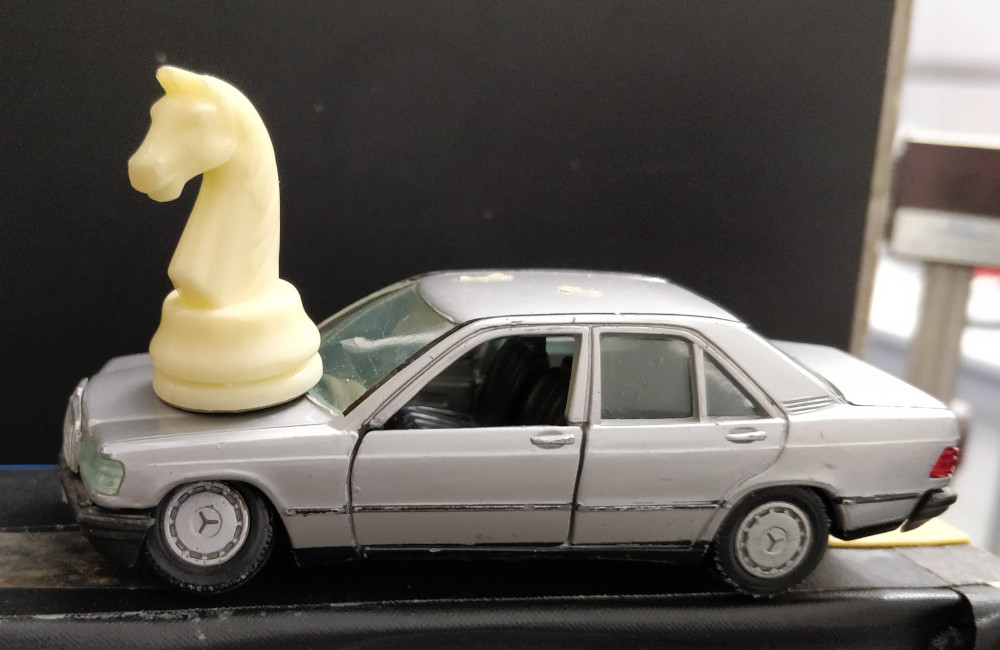
\includegraphics[width=\textwidth]{car_knight}
\caption{Object}
\label{fig:car_knight1}
\end{subfigure}
\begin{subfigure}[b]{0.45\textwidth}
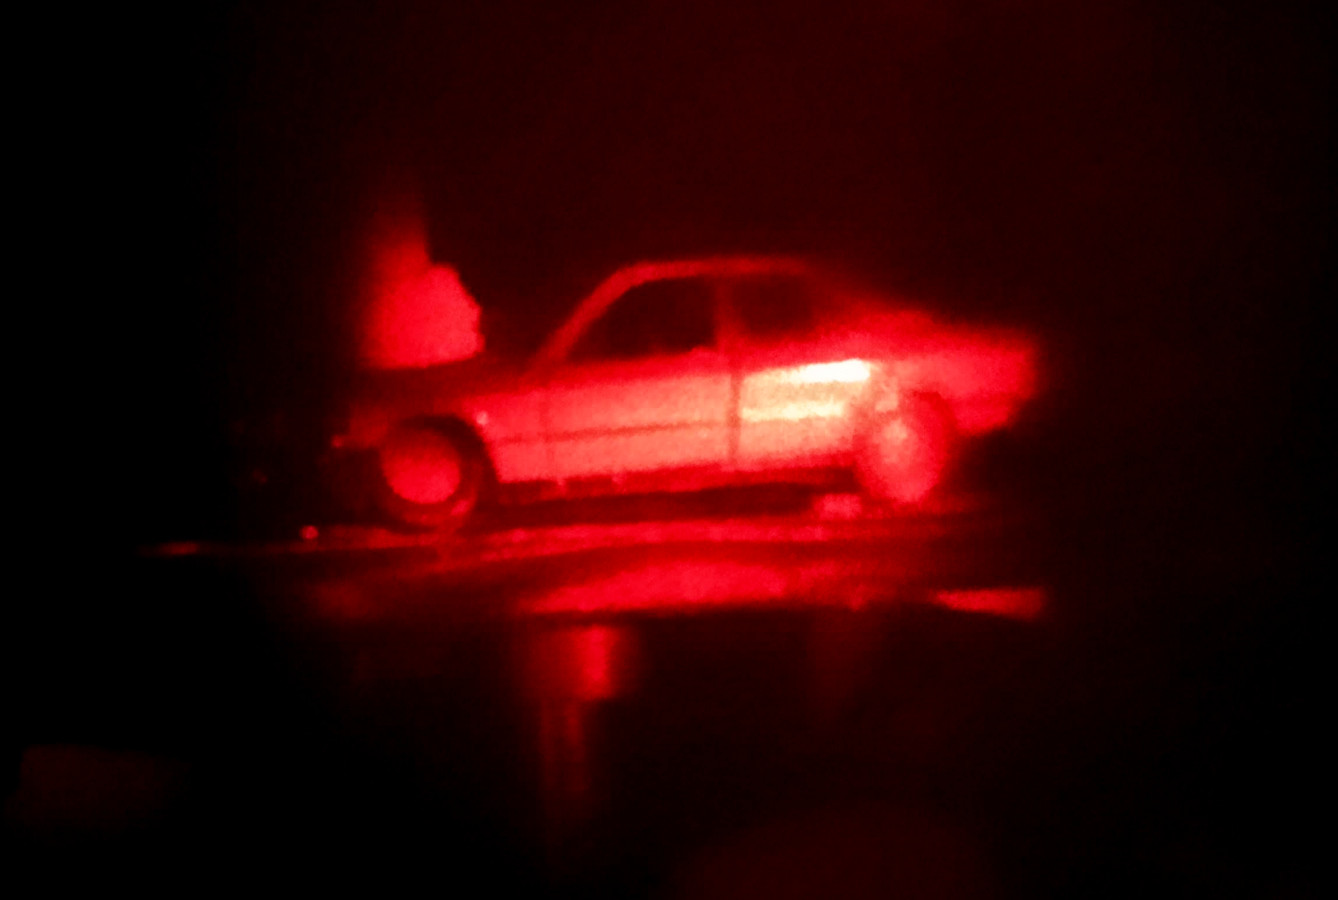
\includegraphics[width=\textwidth]{Off-axis_hologram}
\caption{Hologram}
\label{fig:off_axis_hologram1}
\end{subfigure}
\caption{Off-axis exposure of a car with a knight chess piece on the bonnet. On the left, a picture of the original object. On the right, a picture of the obtained hologram.}
\label{fig:off-axis_exposure}
\end{figure}

The second hologram (Figure \ref{fig:holographic_interferometry_position}) was made with a double exposure of a metallic piece in two different positions. As explained in subsection~\ref{sec:Holo}, we are able to extimate with good precision the distance between the two positions.

\begin{figure}[ht]
\centering
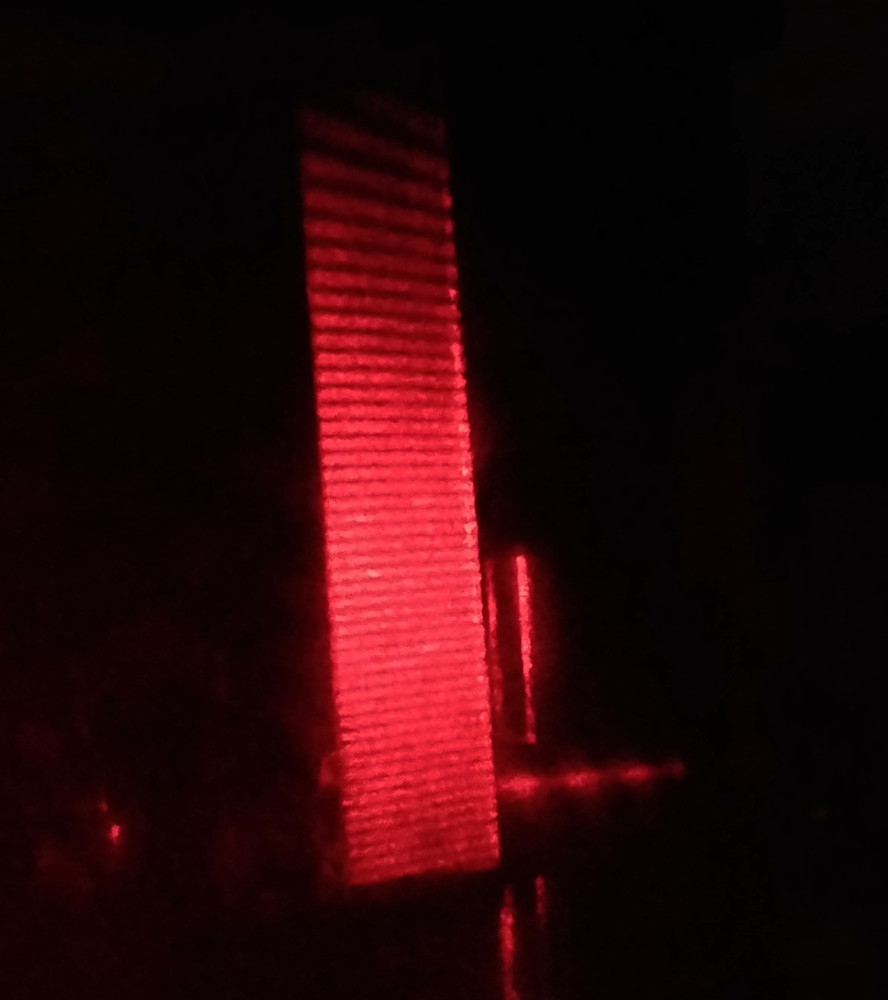
\includegraphics[width=0.5\textwidth]{Holographic_interferometry_position}
\caption{Picture of an hologram with an interference pattern caused by the movement of the metallic piece $\approx\SI{14}{\micro \m}$ between exposures.}
\label{fig:holographic_interferometry_position}
\end{figure}

\begin{figure}[ht]
\centering
\begin{subfigure}[b]{0.4\textwidth}
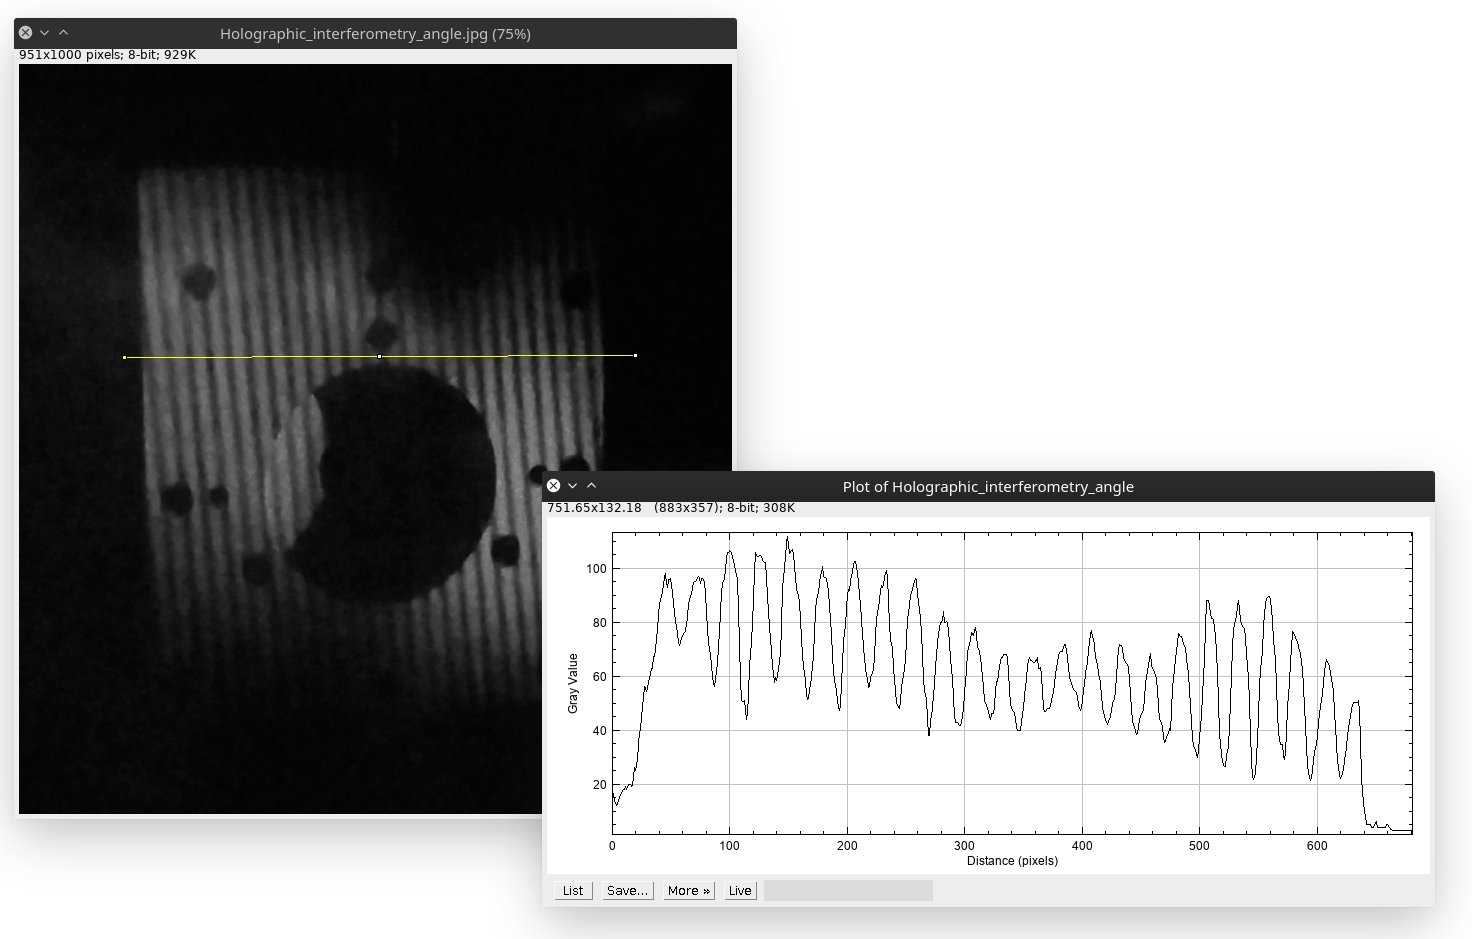
\includegraphics[width=\textwidth]{Holographic_interferometry_angle_fringes}
\caption{}
\label{fig:holographic_interferometry_angle_fringes}
\end{subfigure}\\\vspace{.1cm}
\begin{subfigure}[b]{0.4\textwidth}
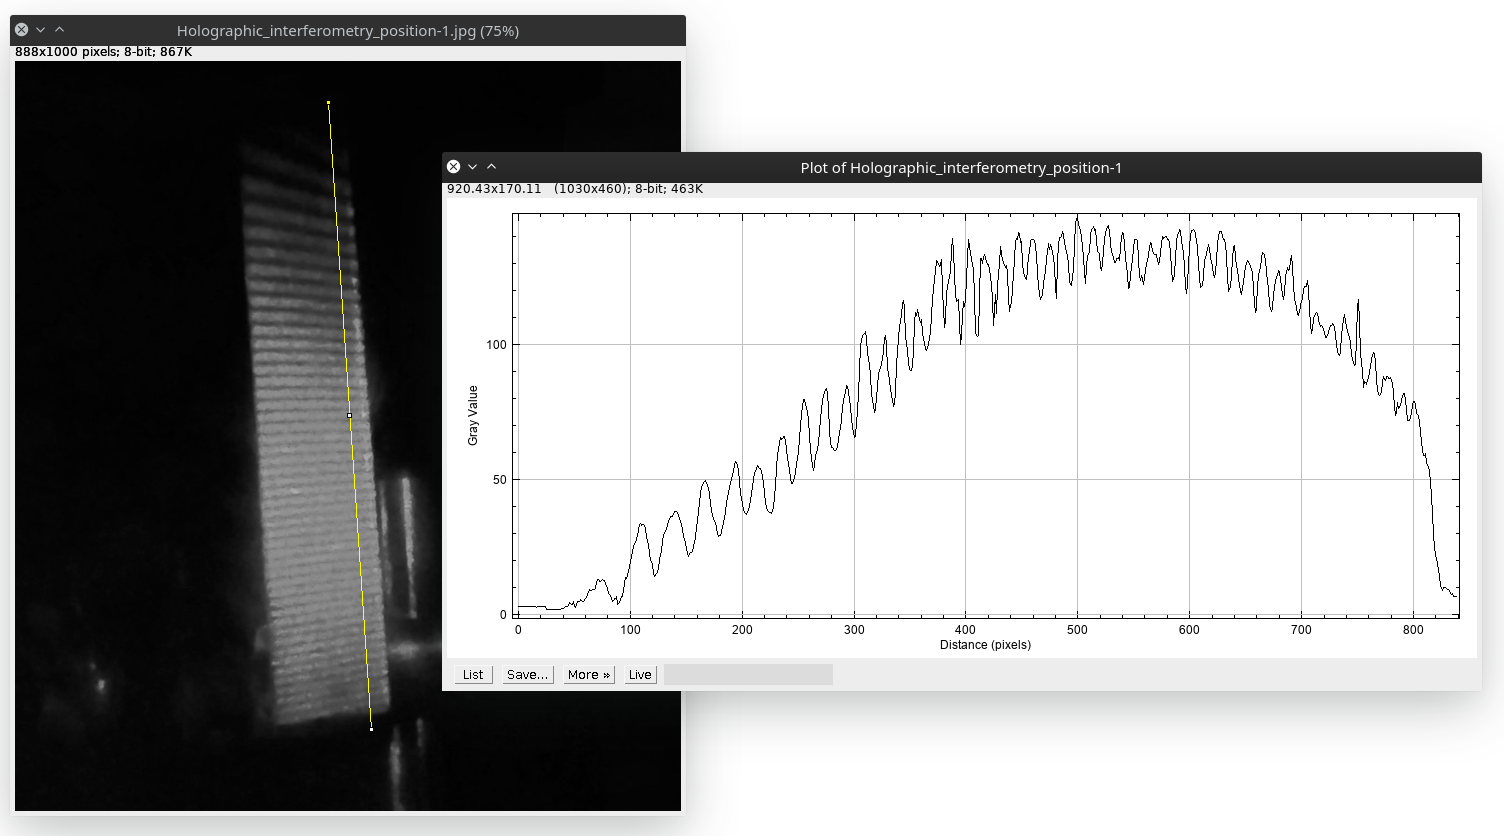
\includegraphics[width=\textwidth]{Holographic_interferometry_position_fringes}
\caption{}
\label{fig:holographic_interferometry_position_fringes}
\end{subfigure}
\caption{In \ref{fig:holographic_interferometry_angle_fringes}, the profile along the horizontal direction (yellow line). In \ref{fig:holographic_interferometry_position_fringes}, the profile along the vertical direction (yellow line). Peaks correspond to constructive interference and by counting them we get the number of fringes.}
\label{fig:profile_measurements}
\end{figure}

Knowing the wavelenght of the laser ($\lambda=\SI{632.8}{\nano\m}$), the angles formed by the laser beam and the normal to the object ($\theta_1 =29^\circ \pm 5^\circ$ and $\theta_2 =30^\circ \pm 5^\circ$) and number of fringes ($N=48 \pm 2$, as we can see from Figure~\ref{fig:holographic_interferometry_position_fringes}), we can compute the distance $d$ using equation~(\ref{eq:d}). The result obtained is: $d \simeq \SI{17}{\micro\m}$.

In the same way, we evaluate the uncertainty of this measurement using the propagation of uncertainty. We obtain: $\Delta d=\SI{2}{\micro\m}$.

Third hologram (Figure \ref{fig:holographic_interferometry_angle}) was again a double exposure of a piece of metal, but now before and after a small rotation (of an angle $\alpha$). As explained in subsection~\ref{sec:Holo}, it is possible to extimate with good precision our $\alpha$.

\begin{figure}[ht]
\centering
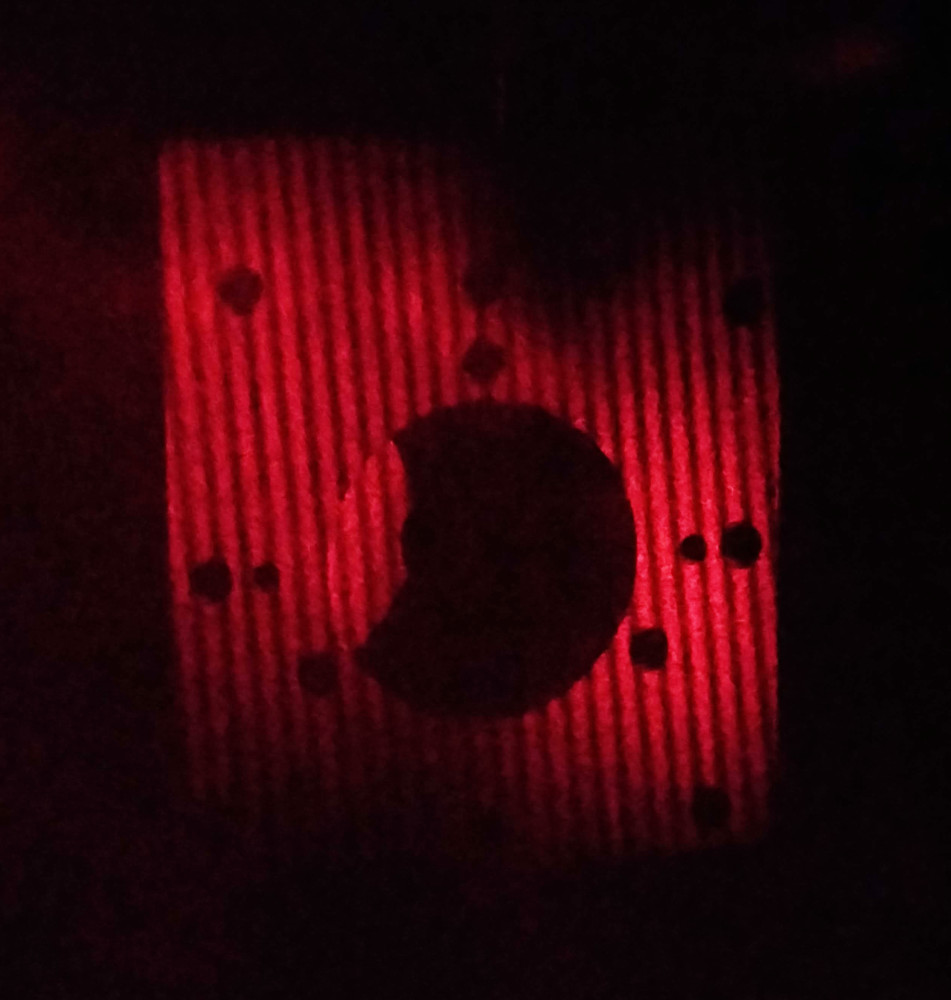
\includegraphics[width=0.4\textwidth]{Holographic_interferometry_angle}
\caption{Picture of an hologram with an interference pattern caused by the rotation of the metallic piece $\approx (1/72)^\circ$ between exposures.}
\label{fig:holographic_interferometry_angle}
\end{figure}

Using equation~(\ref{eq:alp}) and knowing $R=\SI{7.8\pm0.1}{\cm}$, $N=25\pm 2$ (as we observe in Figure~\ref{fig:holographic_interferometry_angle_fringes}), $\lambda=\SI{632.8}{\nano\m}$, $\theta_1=46^o\pm 5^o$ and $\theta_2=11^o\pm 5^o$, we get to the result: $\alpha= 0.0130^o\pm 0.0009^o$.


During the experiment, we have tried to roughly measure the distance $d$ and the angle $\alpha$. The distance was $d\sim 14\mu m$, so in good accordance with the result obtained. As far as the angle is concerned, we know that we moved the wheel a bit less then 1 step, where every step was $\frac{1}{72}^o\simeq 0.0139$; therefore we can conclude that even in this case the measurement agrees with the extimated value of the angle.

Finally, we tried to do a second hologram where we wanted to create the effect of a superposition of the bonnet of two cars travelling in opposit direction (Subfigure~\ref{fig:dir1} and \ref{fig:dir2}). Unfortunately, the time of exposure was not enough and the result has been unsatisfying as we can see from subfigure~\ref{fig:result}.

\begin{figure}[ht]
\centering
\begin{subfigure}[b]{0.45\textwidth}
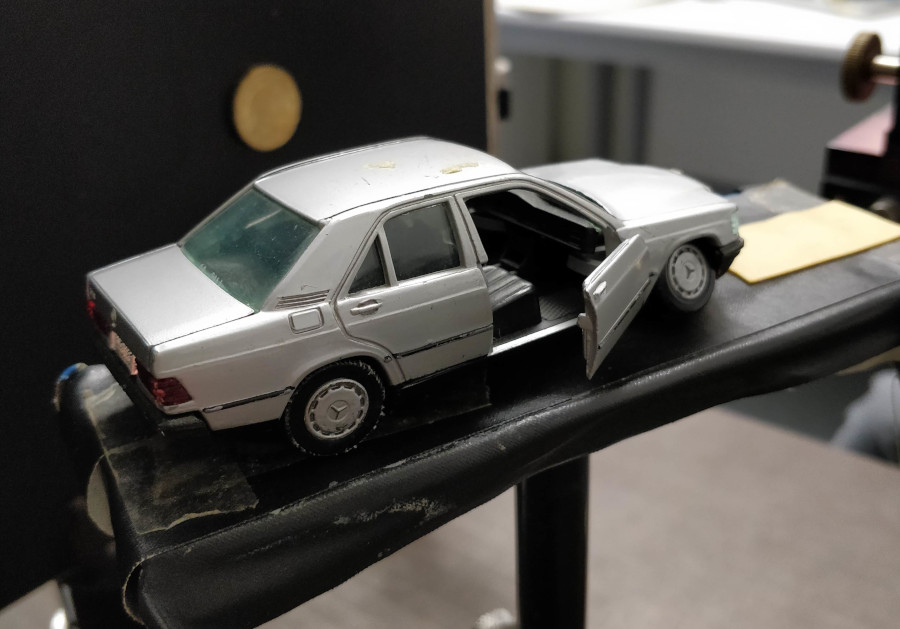
\includegraphics[width=\textwidth]{car_double_exposure_1}
\caption{Position first exposure}
\label{fig:dir1}
\end{subfigure}
\begin{subfigure}[b]{0.45\textwidth}
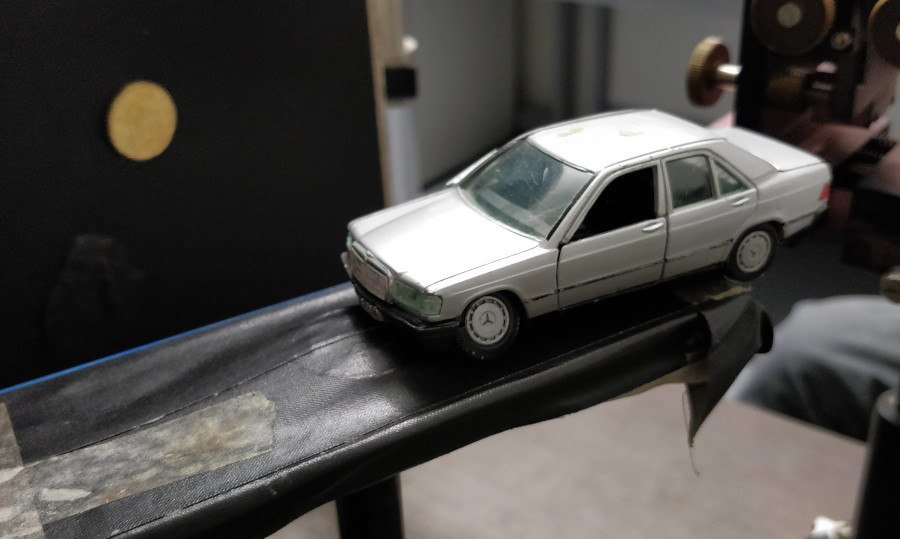
\includegraphics[width=\textwidth]{car_double_exposure_2}
\caption{Position second exposure}
\label{fig:dir2}
\end{subfigure}\\\vspace{.2cm}
\begin{subfigure}[b]{0.35\textwidth}
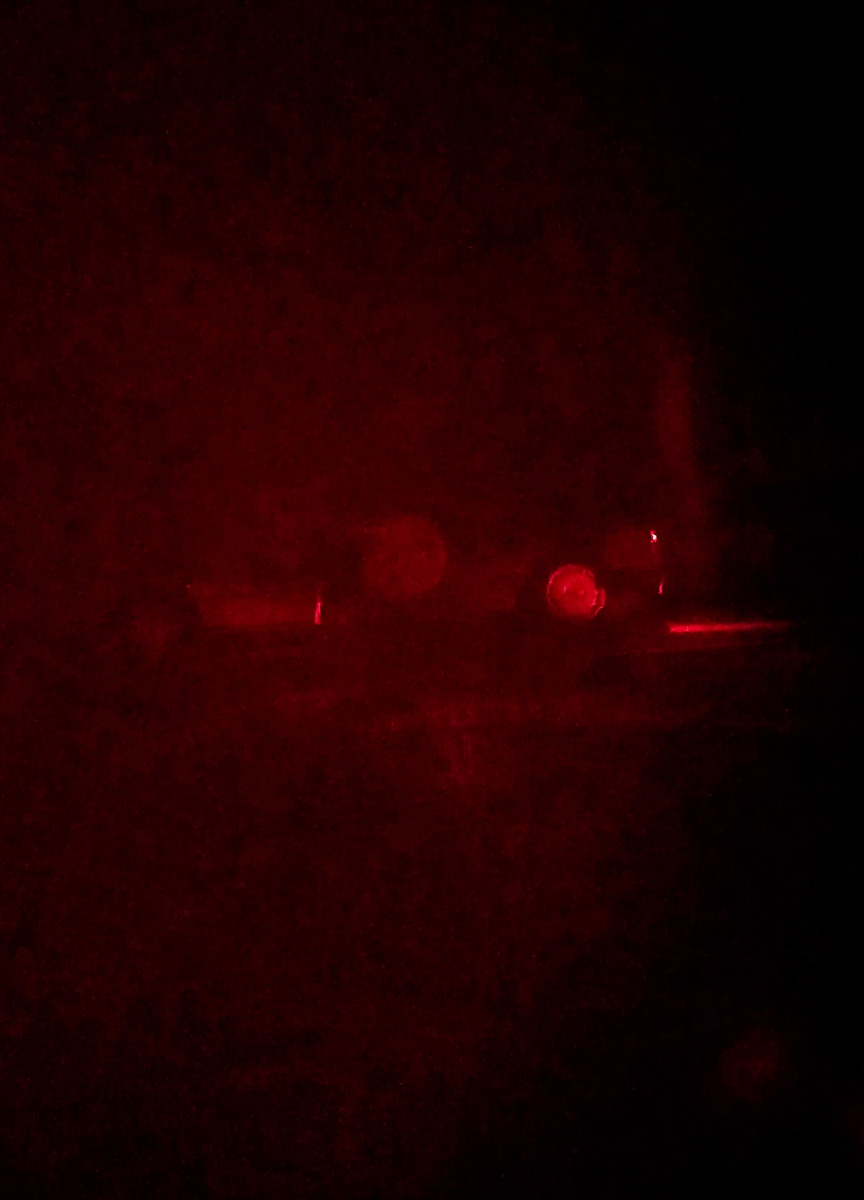
\includegraphics[width=\textwidth]{car_double_exposure_hologram}
\caption{Picture of the obtained hologram}
\label{fig:result}
\end{subfigure}
\caption{Setup and hologram of a double \SI{45}{\second} exposure in which we moved and rotated the car between exposures.}
\label{fig:experiment_double_exposure}
\end{figure}

\vfill
\nocite{*}
\bibliographystyle{unsrt}
\bibliography{references}
\end{document}